%------------------------------------------%
%
% Cannabis Data Science #60
%
% Date: 4/6/2022
%
%------------------------------------------%
\documentclass[xcolor={dvipsnames}]{beamer}
\hypersetup{pdfpagemode = FullScreen}
\mode<presentation>{
  \usetheme{Boadilla}
  \usecolortheme{orchid}
  \usefonttheme{default}
  \setbeamertemplate{navigation symbols}{}
  \setbeamertemplate{caption}[numbered]
}
\setbeamersize{
  text margin left = 0.5in,
  text margin right = 0.5in
}

%------------------------------------------%
% Title
%------------------------------------------%
\title[\textbf{Cannabis Data Science \#60}]{}
\author{Cannlytics}
\institute[]{\Large Cannabis Data Science \#60}
\date{April \nth{6}, 2022}

%------------------------------------------%
% Packages
%------------------------------------------%
\usepackage[english]{babel}
\usepackage[utf8x]{inputenc}
\usepackage{tikz} % For styling.
\usepackage{xparse}

%------------------------------------------%
% Colors
%------------------------------------------%
\definecolor{Green}{RGB}{34, 153, 84}
\definecolor{LightGreen}{RGB}{218, 247, 166}
\definecolor{DarkGreen}{RGB}{2, 48, 32}
\definecolor{Orange}{RGB}{255, 87, 51}
\definecolor{DarkOrange}{RGB}{199, 0, 57}
\definecolor{Yellow}{RGB}{255, 195, 0}

%------------------------------------------%
% Theme
%------------------------------------------%
\setbeamercolor*{palette primary}{bg=LightGreen, fg=DarkGreen}
\setbeamercolor*{palette secondary}{bg=LightGreen, fg=DarkGreen}
\setbeamercolor*{palette tertiary}{bg=LightGreen, fg=DarkGreen}

%------------------------------------------%
% Packages
%------------------------------------------%
\usepackage{amsmath}
\renewcommand*\footnoterule{} % No separating line on footnote.
\usepackage{mathtools} % For annotating equations.
\usepackage{hhline} % for double bars.
\usepackage[super]{nth} % For formatting 1st, 2nd, 3rd, etc.
\usepackage{graphicx, caption, subcaption}
\usepackage{setspace}

%------------------------------------------%
% Commands
%------------------------------------------%

% Top space.
\newcommand\T{\rule{0pt}{2.5ex}}

% Bottom space.
\newcommand\B{\rule[-1.25ex]{0pt}{0pt}}

% Blocks.
\newenvironment<>{Block}[2][.9\textwidth]
  {\setlength{\textwidth}{#1}
  \begin{actionenv}#3
    \def\insertblocktitle{#2}\par
    \usebeamertemplate{block begin}}
  {\par\usebeamertemplate{block end}
  \end{actionenv}}

% Balls.
\defbeamertemplate{enumerate item}{largeball}
{\begin{pgfpicture}{-1ex}{-0.65ex}{1.5ex}{1.5ex}
\usebeamercolor[fg]{item projected}
{\pgftransformscale{2.5}\pgftext{\Large\pgfuseshading{bigsphere}}}
{\pgftransformshift{\pgfpoint{0pt}{0.5pt}}
\pgftext{\usebeamerfont*{item projected}\small\insertenumlabel}}
\end{pgfpicture}}

% Fancy arrows.
\NewDocumentCommand\UpArrow{O{2.0ex} O{black}}{%
   \mathrel{\tikz[baseline] \draw [->, line width=0.5pt, #2] (0,0) -- ++(0,#1);}} % Fancy up-arrow.
\NewDocumentCommand\DownArrow{O{2.0ex} O{black}}{%
   \mathrel{\tikz[baseline] \draw [<-, line width=0.5pt, #2] (0,0) -- ++(0,#1);}} % Fancy down-arrow.

% Equations with numbers on the left.
\makeatletter
\newcommand{\LeftEqNo}{\let\veqno\@@leqno}
\makeatother


\defbeamertemplate*{title page}{customized}[1][]
{
  \usebeamerfont{title}\inserttitle\par
%  \usebeamerfont{subtitle}\usebeamercolor[fg]{subtitle}\insertsubtitle\par
  \bigskip
  \vspace{0.5\baselineskip}
  \usebeamerfont{institute}\insertinstitute\par
  \vspace{0.5\baselineskip}
  {\small\usebeamerfont{date}\insertdate\par}
  \usebeamercolor[fg]{titlegraphic}\inserttitlegraphic
}

%------------------------------------------%
%
% Presentation
%
%------------------------------------------%
\begin{document}

% Title page.
\begin{frame}{}

% Background
\tikz[remember picture, overlay]
\node[opacity=1.0, inner sep=0pt] at (current page.center){
  
\includegraphics[height=\paperheight, width=\paperwidth]{images/presentation-cover.pdf}
};

% Title
\vspace*{3\baselineskip}

\includegraphics[scale=0.375]{images/logo.pdf}
\vspace*{-2\baselineskip}
\titlepage
  
\end{frame}

%------------------------------------------%
% Introduction
%------------------------------------------%

\begin{frame}{}

\vspace{1\baselineskip}
\begin{center}
\begin{minipage}{0.85\textwidth}

{\itshape `` {\bfseries Utility} analysis is a highly theoretical construct ... to serve as a link in the chain connecting human \underline{preferences} with economic \underline{behavior}.''}

\vspace{-0.25\baselineskip}
\begin{flushright}
\begin{minipage}{0.7\textwidth}

\tiny

-  Martin Weitzman,\\{\itshape Utility Analysis and Group Behavior: An Empirical Study} (2008).

\end{minipage}
\end{flushright}

\end{minipage}
\end{center}


\vspace{0.5\baselineskip}
\begin{center}
\begin{minipage}{0.6\textwidth}
\begin{figure}
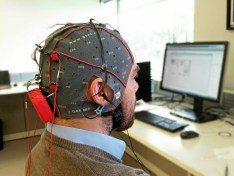
\includegraphics[width=2.25in]{images/eeg-neurotech.jpg}
\caption*{%
\small A neurological measurement device.\\[0.25\baselineskip]
\tiny\color{Gray} Author: William Broek\\
License: CC BY-SA 4.0 https://creativecommons.org/licenses/by-sa/4.0
}
\end{figure}
\end{minipage}
\end{center}

% Reading:
% https://adcare.com/massachusetts/marijuana/

\end{frame}

%------------------------------------------%
% Utility Functions
%------------------------------------------%

\begin{frame}{Utility}

\begin{itemize}

\item Individuals behave {\bfseries as if} they receive \underline{utility} from {\itshape believing} they have satisfied their \underline{preferences}.

\vspace{1\baselineskip}

\item Utility is generally not compared between individuals.\\
{\tiny{\itshape The Impossibility of Interpersonal Utility Comparisons}, Hausman (1995)}

\vspace{1\baselineskip}

\item Utility maximazation is found by maximizing the Lagrangian

\vspace{-0.5\baselineskip}
$$
\mathcal{L} = \mathcal{U}(x, \alpha) + \lambda(I - p_x \cdot x)
$$

\vspace{0.5\baselineskip}
where utility is maximized at consumption set $x^*$ given \underline{prices}, $p_x$, and a consumer's \underline{preferences}, $\alpha$.

\end{itemize}

% Johnny von Neumann contribution to solve 


% Ethnicity -> Cofounding factor?

\end{frame}

%------------------------------------------%
% Consumer Choice
%------------------------------------------%

\begin{frame}{Consumer Choice}

\begin{minipage}{0.445\textwidth}

{\bfseries Consumers} are people who purchase your product.

\vspace{1\baselineskip}

{\bfseries Potential consumers} are

\vspace{0.5\baselineskip}
\begin{itemize}

\item Those interested in purchasing, who haven't.

\vspace{0.5\baselineskip}

\item Those that purchase a substitute product.

\vspace{0.5\baselineskip}

\item Those using illicit avenues.

\end{itemize}

\end{minipage}\hspace{0.05\baselineskip}
\begin{minipage}{0.5\textwidth}

\begin{figure}
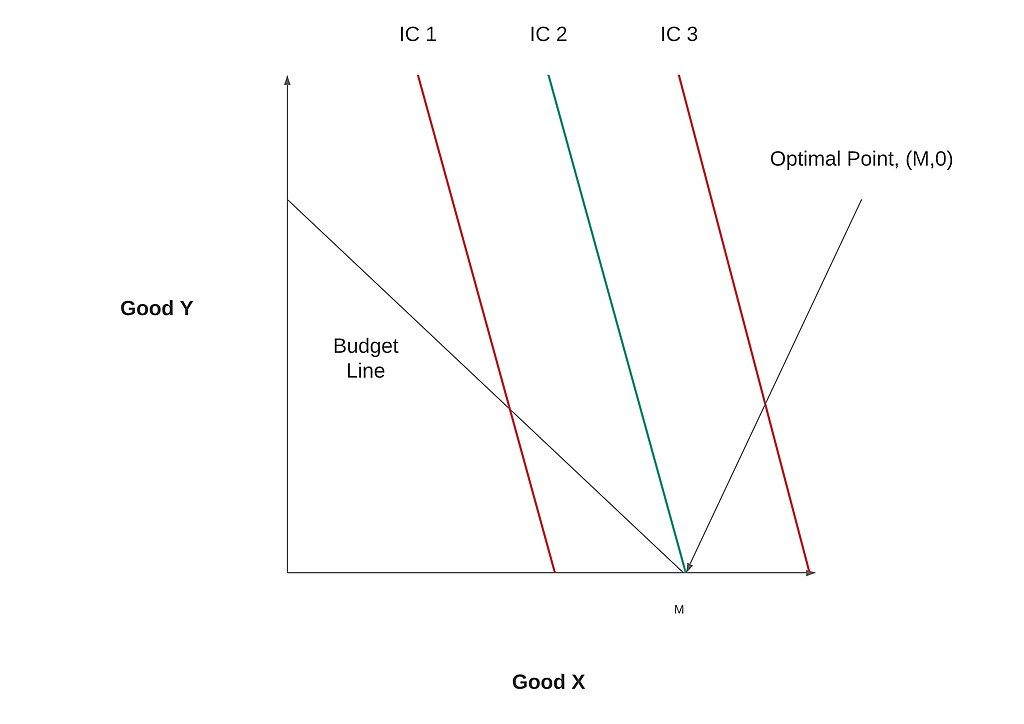
\includegraphics[width=\textwidth]{images/corner-solution.jpg}
\caption*{%
\hspace{2.5ex}\tiny A corner solution withe optimal bundle $(M, 0)$.\\
\tiny\color{Gray}
\hspace{4ex}Author: Stephanosg\\
\hspace{4ex}License: CC BY-SA 4.0\\
\hspace{4ex}https://creativecommons.org/licenses/by-sa/4.0
}
\end{figure}

\end{minipage}

\end{frame}

% More is better.

% When people talk about different types of consumers, economists think different indifference curves.

% The indifference between all goods plays a role in a consumer's choice.

% Income effect.

% Expectations.

% Time preferences.

% E.g. some people view peanut butter and jelly as compliments and some view them as substitutes.


% Imperfect substitutes

% Loyalty

% Learning

% Variety seeking

% There is an analytics company, worth 350+ million, selling biased statistics at around $300-$600 per month.
% Inconsistent and biased. People can at least make decisions.


%------------------------------------------%
% A Sprinkle of Economics (excluded for time?)
%------------------------------------------%
%\section{A Brief Sprinkle of Economics}
%\begin{frame}{A Sprinkle of Economics: Competing for Profits}
%
%\vspace*{0.125\baselineskip}
%
%Market Effects
%
%- Michael Porter
%
%Competitive rivalry
%
%  - Degree of advertising
%  - Competitive Advantage / Comparative Advantage
%
%Buyer power
%
%  - Buyer concentration to firm concentration ratio
%  - Price elasticity of demand.
%
%Supplier power
%
%  - Input costs
%
%Threat of new entry
%
%Threat of substitution
%
%Observe:
%
%Markets of substitute goods tend to experience great volatility in prices, driving down producer profits.
%
%Prices tend to be reduced in attempts of producers to capture market share.
%
%Consumers may be able to attain more utility when there are available substitute products.
%
%In interdependent markets, game theory must be used to derive a profit maximizing solution.
%
%%\begin{itemize}
%%
%%\item Cournot
%%
%%\item Joseph Bertrand
%%
%%\item Pareto
%%
%%\item Irving Fisher
%%
%%\end{itemize}
%
%\end{frame}

% TODO: Talk about sbustitutes in production.


% TODO: Correlate concentration ratio for various product types and the vendors total sales (hue by producer type).

% that can produce cannabis products as {\bfseries substitutes in production}


%\begin{itemize}
%
%\item It is easier to argue that there is natural variance in products such as flower, however, the ability for a beverage manufacturer to capture a large section of the market given a uniform product, typically a 100mg beverage, may depend largely on their marketing effectiveness.
%
%\item Do encumbants get market share?
%
%\item Run the gamut with beverage brand analysis.
%
%\item Using beverage product type for simplicity. The analysis can be readily applied to all product types.
%
%\end{itemize}


%------------------------------------------%
% Scientific Method
%------------------------------------------%

\begin{frame}{Our Scientific Method}

\begin{enumerate}

\item Experimental design: based on prior research.

\vspace{1\baselineskip}

\item Hypothesis generation: record!

\vspace{1\baselineskip}

\item Collect data.

\vspace{1\baselineskip}

\item Test our hypothesis.

\vspace{1\baselineskip}

\item Reproduce.

\end{enumerate}

\end{frame}


%------------------------------------------%
% Question and Hypothesis
%------------------------------------------%
\section{Question and Hypothesis}
\begin{frame}{Question and Hypothesis}

% Question of the day
\begin{center}
\begin{minipage}{.9\linewidth}
\begin{Block}{Question of the day.}

\vspace{.5\baselineskip}
\begin{itemize}

\item How does the \underline{price} of other goods affect cannabis consumption?

\vspace{1\baselineskip}

\item How will \underline{inflation} affect the {\bfseries proportion} of people using cannabis and the {\bfseries quantity} of cannabis consumed by people who consume cannabis?

\end{itemize}

\vspace{.5\baselineskip}

\end{Block}
\end{minipage}
\end{center}

\vspace{1.5\baselineskip}
These are questions that the Cannabis Data Science group is uniquely positioned to answer.

\end{frame}


%------------------------------------------%
% Saturday Morning Statistics Promo
%------------------------------------------%
\begin{frame}{Coming up in Saturday Morning Statistics}

\begin{itemize}

\item Logit, Probit, and Tobit model extensions!

\vspace{1\baselineskip}

\item Heckman (1981) showed that estimating choice models based on observed choices may lead to strong state dependence {\itshape if} \underline{participation} is not modeled.

\vspace{1\baselineskip}

\item Heckman-selection (Tobit Type II) models can correct for selection bias and yield {\bfseries unbiased} and {\bfseries consistent} estimates, even when the proportion of missing data is substantial.

\end{itemize}

\end{frame}


%------------------------------------------%
% Takeaway
%------------------------------------------%
\section{Takeaway}
\begin{frame}{}

\begin{center}
\begin{minipage}{3.85in}

% Thank you.

\includegraphics[width=.25in]{images/prayer.png} {\Large \textbf{Thank you for coming.}}\\[-0.5\baselineskip]

\begin{center}
\begin{minipage}{\linewidth}
\begin{Block}{Insight of the Day}

\vspace{0.5\baselineskip}

\begin{itemize}

\item Modeling both \underline{participation} and \underline{consumption} is critical in making {\bfseries unbiased}, {\bfseries consistent} predictions in the cannabis industry.

\vspace{0.5\baselineskip}

\end{itemize}

\end{Block}
\end{minipage}
\end{center}

\vfill

\end{minipage}
\end{center}

\vspace{0.5\baselineskip}

In Saturday Morning Statistics this week, we will do just that. What would you like to talk about next week?

\vspace{0.5\baselineskip}

\end{frame}


%------------------------------------------%
% Fin.
%------------------------------------------%
\end{document}
